% Background chapter continued..

\section{Evaluation Metrics for Recommendation Systems}

In this section we will see few of these methods that are used as evaluation metrics for recommender systems algorithms. Evaluation can be done by two ways, offline and online evaluation \cite{22,23}. In offline analysis collected data is divided into train set and test set in proportion of 80 to 20. The model of recommender system is trained on train dataset and test dataset is hidden from engine. Afterwords build algorithm trained on train dataset is used to predict ratings of unseen items. To understand the quality of recommendation engine, one or combination of evaluation metrics are used. There are several methods available to evaluate the performance of the recommender systems \cite{22,24}. We will see discuss those methods as follow. 
  
\subsection{Recall and Precision}

Recall and precision are most commonly used metrics to evaluate recommendation engines \cite{25}. These metrics can be explained by a confusion matrix \cite{21} as shown in \autoref{fig:confusion_matrix}.
  
\begin{figure}[H]
	\centering
	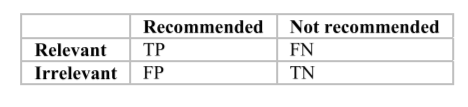
\includegraphics[width=0.7\linewidth]{confusion_matrix}
	\caption{Confusion matrix for calculating recall and precision \cite{21}.
	\label{confusion_matrix} }
	\label{fig:confusion_matrix}
\end{figure}

Where\\
TP denotes True Positive represents all relevant items are recommended by the system.\\
TN denotes True Negative represents all irrelevant items are correctly not recommended by the system.  \\
FP denotes False Positive represents all irrelevant items which are
incorrectly recommended by the system\\
FN denotes False Negative represents relevant items but system failed to recommend.\\
Based on \autoref{confusion_matrix}, precision is calculated as ratio of the relevant items from recommended items to the number of all recommended items. It is given in \autoref{eq:precision}. 

\begin{equation}
Precision = \frac{TP}{TP + FP} 
\label{eq:precision}
\end{equation}

Based on \autoref{confusion_matrix}, recall is calculated as the ratio of relevant items from recommended items to the number of all relevant items. It is given in \autoref{eq:recall}. 

\begin{equation}
Pecall = \frac{TP}{TP + FN} 
\label{eq:recall}
\end{equation}

--------- To DO ---------
\subsection{Root Mean Squared Error (RMSE)}
--------- To DO ---------
\subsection{Mean Reciprocal Rank}
--------- To DO ---------
\subsection{MAP at k (Mean Average Precision at cutoff k)}
--------- To DO ---------
\subsection{NDCG (Normalized Discounted Cumulative Gain)}
--------- To DO ---------